\begin{figure}
 \centering  % this centres figure in column
  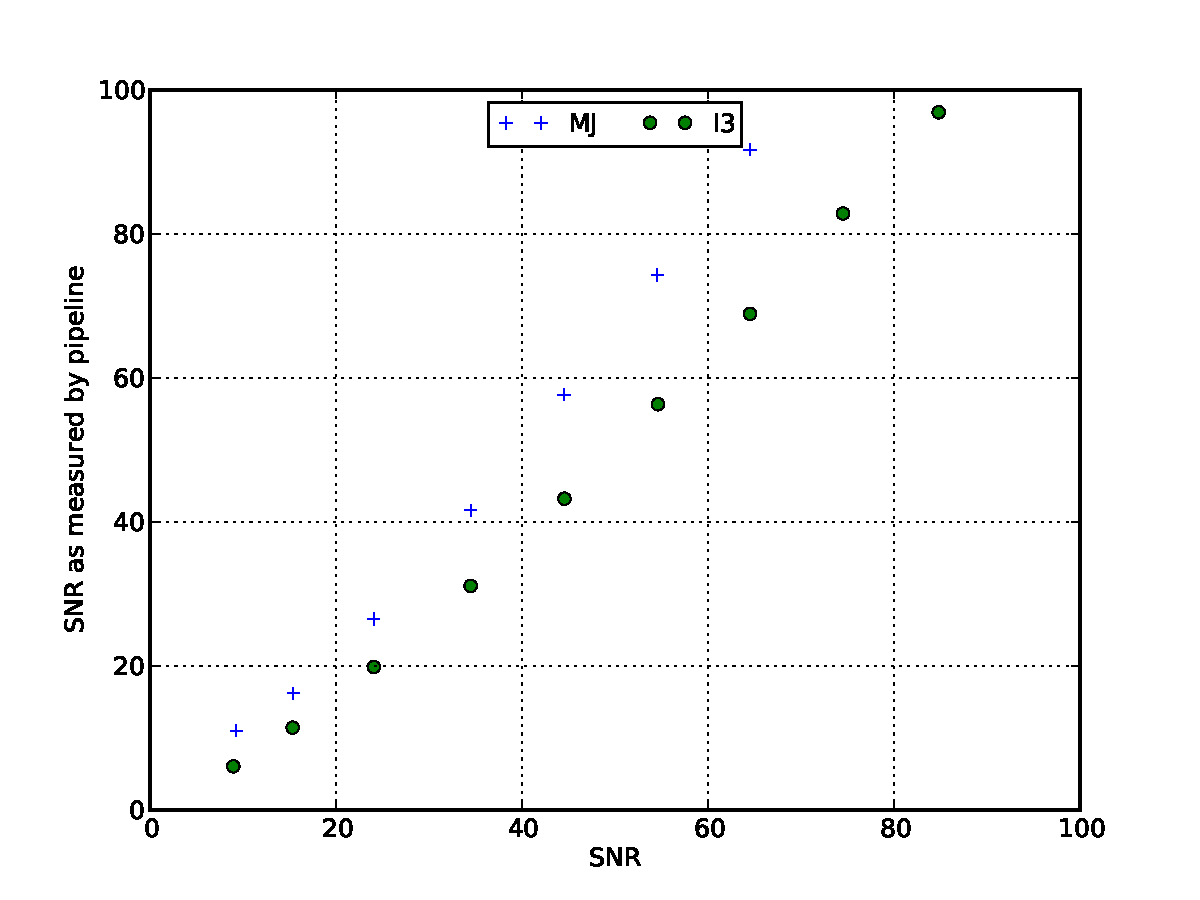
\includegraphics[width=0.5\textwidth]{fig/SNR_mfix.pdf} 
  \caption{The measurement of Signal-to-Noise Ratio (SNR) as defined
    in (cf Eqn.~\ref{Eqn:SNR_ref}) versus the SNR as measured by the
    individual pipelines.}
\label{fig:Snr_comp}
\end{figure}

The level of pixel noise present in galaxy images
greatly impacts the ability of lensing pipelines 
to accurately measure shear \citep[e.g.][]{peter_n, Okura_n, R_n}. 
The multiplicative bias due to pixel noise varies 
depending on both the source galaxy population
and the lensing pipeline. There have been a number
of calibration schemes that attempt to correct for the
effect of noise bias for specific lensing pipelines developed
including \citep{K_n} and \citep{cfhtls} on previous image 
simulations.  \\
\indent The Signal-to-Noise Ratio (SNR) was measured on the CSTEP images
for each galaxy using the Source Extractor software package 
\citep{Sext} with SNR defined as  
\begin{equation}\label{Eqn:SNR_ref}
SNR = \frac{\textrm{Flux}}{\textrm{Flux Error}}
\end{equation}
and where the flux was determined using automatic apertures.  A
comparision of the SNR as measured by Source Extractor and as measured
by the individual pipelines is shown in \ref{fig:Snr_comp}. 

To make the results easier to interpret and compare to previous
studies, the bias of the lensing pipelines was quantified in this
section by a linear function
\begin{equation}
\gamma_m = (m+1) (\gamma_t) + c
\end {equation}
where again $\gamma_t$ is the true shear and $\gamma_m$ is the measured shear.
The results of the multiplicative bias as a function of SNR are shown in Figure \ref{fig:Snr}. 
\begin{figure}
 \centering  % this centres figure in column
  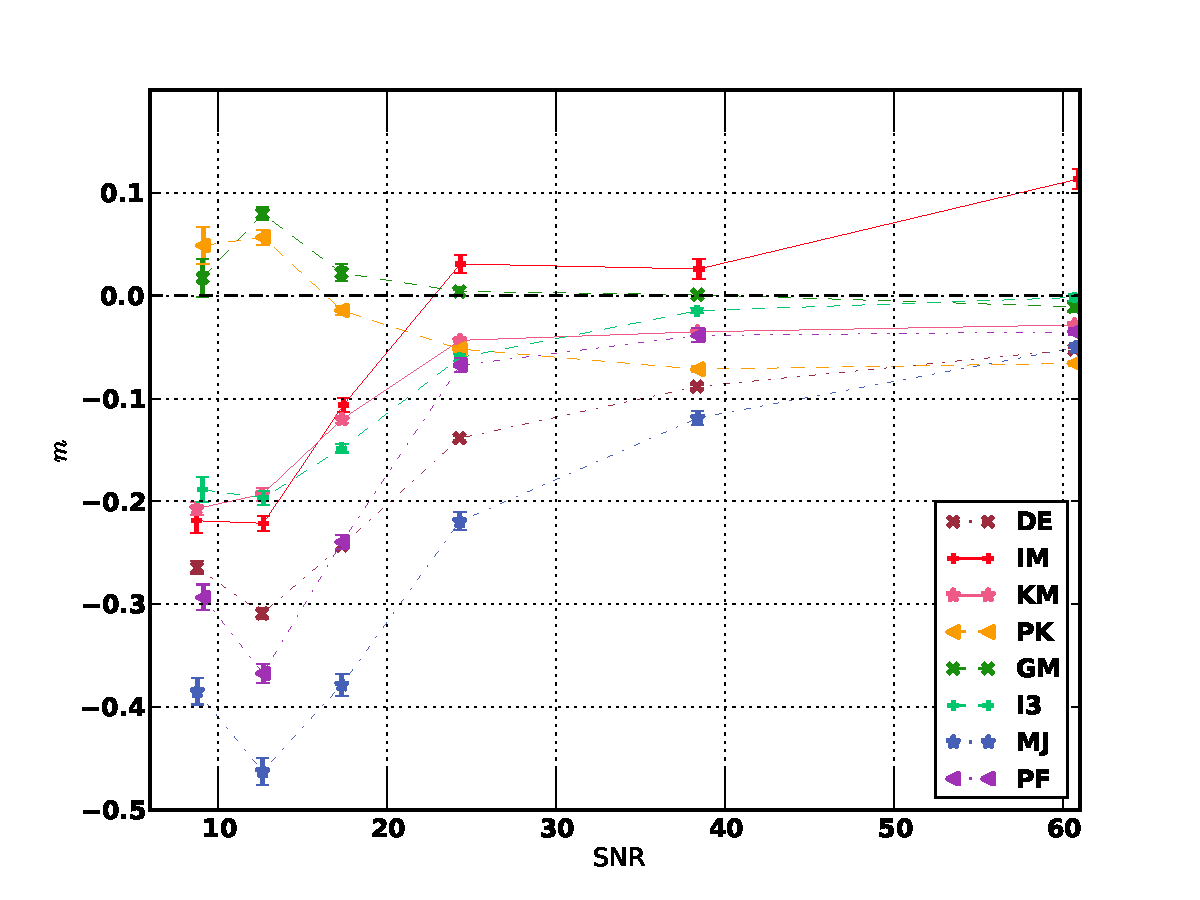
\includegraphics[width=0.5\textwidth]{fig/MvalSNR_v2.pdf} 
  \caption{Multiplicative bias ($m$) as a function
    of Signal-to-Noise Ratio (SNR). The multiplicative bias was determined
    using a linear fit of measured to true mean shear.}
\label{fig:Snr}
\end{figure}

